\chapter{Software Development}
\label{chap:software-development}

\section{Software Development Methodology}
\label{section:software-development-methodology}
<TIP: Describe your software development methodology in this section. />
Extreme Programming (XP)
In short, it is -
-Extreme programming (XP) is an Agile project management methodology that targets speed and simplicity with short development cycles. XP uses five guiding values, five rules, and 12 practices for programming. The structure is rigid, but the result of these highly focused sprints and continuous integrations can result in a much higher quality product.

- asana's summary of XP 

By definition, XP is ...

In this project's case,


has 3 professor to overview work consistently
2 people project
fixed deadlines
4 months project work time in total
consistent testing
single codebase


\section{Technology Stack}
\label{section:technology-stack}
<TIP: Describe your technology stack here. See the following example from ThaiProgrammer.org />
\begin{figure}[h]
    \centering
    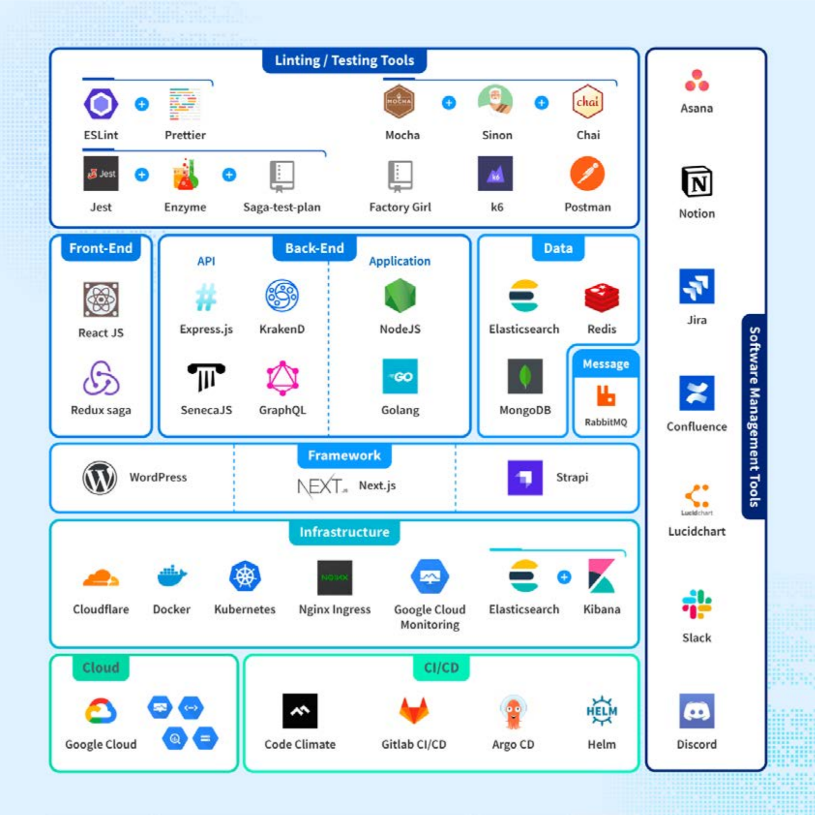
\includegraphics[width=0.5\textwidth]{examples/tech-stack.png}
    \caption{Example technology stack}
\end{figure}

\section{Coding Standards}
\label{section:coding-standards}
<TIP: Describe your coding standard for this project here. />

\section{Progress Tracking Report}
\label{section:progress-tracking-report}
<TIP: Show that you have been working on this project overtime.
It can be in the form of a burndown chart or a contribution graph from GitHub./>
